\scanpage{83}
\mspage{\handwritten{74}}
% One diagonal cancellation crosses all three main text blocks.
\deleted{ment constant à fibres finies et que les ${}_nG^o$ (pour $n\handwritten{\geq}1$) sont des schémas en groupes \deleted{les} finis localement libres sur $S$, que $H$ est fini localement libre sur $S$, et que \handwritten{l}a formation \deleted{commute} de $\underline{\operatorname{Hom}}(\underline{\varnothing}\ ,\ G^{\handwritten{o\natural}})$ commute à\handwritten{q} tout changement de base. Appliquant les mêmes réflexions aux extensions de $\underline{\varnothing}_n$ par $G^o_n$ , on trouve que celles-ci correspondent aux torseurs sous le Groupe $H_n=Hx_SS_n\handwritten{\simeq}\underline{\operatorname{Hom}}(\underline{\varnothing}_n,\ G^o_n)$. Or, $H$ étant fini localement libre sur $S$, on en conclut aussitôt que la \deleted{donnée du} catégorie des torseurs \inserted{$P$} sous $H$ équivaut (par le foncteur ``complétion formelle'') à la catégorie des torseurs sous $\overset{\handwritten{\scriptscriptstyle\wedge}}{H}$ i.e. des``systêmes cohérents'' de torseurs $P_n$ sous les $H_n$ . Cela implique donc que la catégorie des extensions de $\underline{\varnothing}$ par $G^{o\handwritten{\natural}}$ équivaut à celle des \deleted{extensions de} ``systêmes cphérents'' d'extensions des $\underline{\varnothing}_n$ par les $G^o_n$ , ce qui précise donc la définition de l'extension $G^{\handwritten{\natural}}$ de (7.6.1).}

\deleted{Le schéma en groupes $G^{\handwritten{\natural}}$ , en tant qu'extension de $\underline{\varnothing}$ par $G^{o\handwritten{\natural}}$ , dé\uline{\deleted{\unsure{pe}}}pend évidemment encore de façon fonctorielle de $G$. Sa formation est compatible aux changements de base par un morphisme de traits complets $S'\handwritten{\longrightarrow}S$.}

\deleted{7.6.3.Notons que les constructions précédentes gardent également un sens sur une base plus générale qutun \deleted{trait}\inserted{sbhéma \uline{local}} complet; il suffit de partir d'un anneau noethérien adique $\deleted{\unsure{\mathbb{X}|\mathbb{V}}}\handwritten{V}$,\margin{\figure{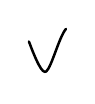
\begin{tikzpicture}[x=1cm,y=1cm]\draw[black,line width=0.9pt,line cap=round,line join=round] (0,0.40) .. controls (0.09,0.16) and (0.17,-0.02) .. (0.22,0.02) .. controls (0.29,0.08) and (0.38,0.45) .. (0.47,0.56);\end{tikzpicture}}} dont la topologie est définie par un \deleted{sché} idéal $\underline{m}\handwritten{\subset}\deleted{\mathbb{X}}\handwritten{V}$, et d'un schéma en groupes $G$ sur $\deleted{\mathbb{X}}\handwritten{V}$ tel que $G_o=G\otimes_{\deleted{\mathbb{X}}\handwritten{V}}\deleted{\mathbb{X}}\handwritten{V}_o$ (où $\deleted{\mathbb{X}}\handwritten{V}_o=\mathbb{X}/\underline{m}$) soit extension d'un schéma en groupes étale fini par un schéma abélien par un \deleted{schéma} tore. La question essentielle est celle de montrer que le schéma formel abélien $\overset{\handwritten{\scriptscriptstyle\wedge}}{B}$\inserted{sur $\deleted{\mathbb{X}}\handwritten{V}$} construit comme dans 7.1 en termes de $G^o$ est algébrisable; cela se voit par la méthode de 7.2 lorsqu'on suppose que $S$ est normal.}
% archive sheet number: 82
